\section{Experimental programme and reproducibility roadmap}

\subsection{A staged research programme}

The lecture should not directly trigger a large end-to-end MMALS redesign. It should generate a ladder of falsifiable experiments.

\begin{figure}[H]
\centering
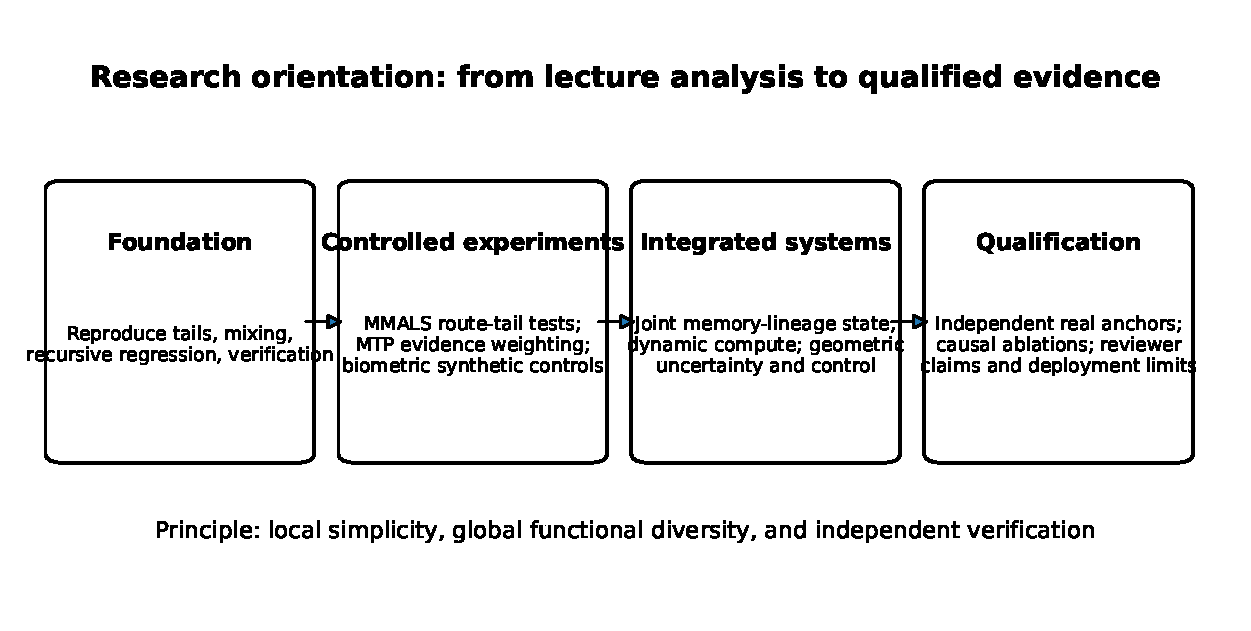
\includegraphics[width=0.97\textwidth]{figures/research_roadmap.pdf}
\caption{Proposed research roadmap.}
\label{fig:roadmap}
\end{figure}

\subsection{Stage 0: reproduce the mathematical mechanisms}

The repository includes lightweight simulations of:

\begin{enumerate}[leftmargin=*]
  \item Hutter scaling under a power-law input distribution;
  \item chopped-tail error floors;
  \item real/synthetic mixing under scarcity;
  \item recursive relabeling;
  \item verifier-based candidate selection.
\end{enumerate}

The objective is not to reproduce every constant from the papers. It is to verify the qualitative signatures:

\begin{itemize}[leftmargin=*]
  \item power-law decrease;
  \item cutoff-dependent plateau;
  \item increased benefit under real-data scarcity;
  \item generational drift under pseudo-label recursion;
  \item recovery when verification enriches correct examples.
\end{itemize}

\subsection{Stage 1: MMALS synthetic-route benchmark}

Construct a controlled problem with known functional regimes. For example:

\begin{itemize}[leftmargin=*]
  \item regime $R_1$: one host is sufficient;
  \item regime $R_2$: a different host is superior;
  \item regime $R_3$: sequential collaboration is necessary;
  \item regime $R_4$: memory is useful;
  \item regime $R_5$: old memory is misleading and must be overridden.
\end{itemize}

Train an initial MMALS version on independently labeled routes, then generate recursive route labels for later versions.

\paragraph{Treatments.}
\begin{enumerate}[leftmargin=*]
  \item real/oracle traces only;
  \item recursive synthetic traces only;
  \item fixed real anchor plus synthetic traces;
  \item accumulated fresh real traces plus synthetic traces;
  \item verified synthetic candidate routes;
  \item lineage-aware consolidation;
  \item dual reconstructive/compiled memory;
  \item state-dependent temperature versus fixed temperature.
\end{enumerate}

\paragraph{Metrics.}
\begin{itemize}[leftmargin=*]
  \item task accuracy and calibrated loss;
  \item final average retention and forgetting;
  \item functional tail coverage;
  \item route entropy and dominance;
  \item host ablation impact;
  \item route-swap degradation;
  \item candidate-permutation sensitivity;
  \item cost per solved input;
  \item number of iterations to convergence;
  \item abstention quality;
  \item synthetic lineage depth;
  \item recovery delay after real anchors are reintroduced.
\end{itemize}

\subsection{Stage 2: verifier bootstrap}

For each input, generate $K$ candidate routes. Let an independent oracle or task residual rank them. Compare:

\begin{itemize}[leftmargin=*]
  \item teacher top-1 route;
  \item oracle best-of-$K$ route;
  \item learned verifier top-1 route;
  \item student trained on accepted routes.
\end{itemize}

A strong result would show:
\[
Q(\text{student}) > Q(\text{teacher top-1})
\]
on an independent real evaluation set, while maintaining or improving functional tail coverage.

The verifier must be audited with:
\[
\phi=\Prob(\text{accept}\mid\text{valid}),
\qquad
\psi=\Prob(\text{accept}\mid\text{invalid}),
\]
stratified by regime and rarity.

\subsection{Stage 3: probabilistic MTP benchmark}

Create a project-level dataset with:

\begin{itemize}[leftmargin=*]
  \item contract and technical-offer features;
  \item preliminary design and dependency structure;
  \item TRL or maturity estimates;
  \item expected margins and resource constraints;
  \item proposed test categories and effort;
  \item defects discovered and production incidents;
  \item source lineage of each observation and test case.
\end{itemize}

Compare four estimators:

\begin{enumerate}[leftmargin=*]
  \item all evidence treated as independent and real;
  \item source-weighted Bayesian model;
  \item hierarchical model with source-specific noise;
  \item lineage-aware model with effective sample-size correction.
\end{enumerate}

Evaluate calibration, posterior coverage, decision regret, residual-risk estimates, and stability under synthetic-data contamination.

\subsection{Stage 4: geometric extension}

Represent covariance, route similarity, or host-state structure on an appropriate manifold. Candidate directions include:

\begin{itemize}[leftmargin=*]
  \item SPD geometry for uncertainty and covariance states;
  \item Stiefel manifolds for learned subspaces;
  \item graph manifolds for dependency or host ecology;
  \item Lie-group state spaces for controlled transformations.
\end{itemize}

The research question is not whether geometric methods are more sophisticated. It is whether they preserve functional distinctions, improve filtering, or provide intrinsic uncertainty bounds that the Euclidean model misses.

\subsection{Ablation discipline}

Every claimed benefit must be compared to the simplest alternative:

\begin{longtable}{p{0.30\textwidth}p{0.58\textwidth}}
\toprule
\textbf{Claimed mechanism} & \textbf{Minimum baseline} \\
\midrule
Synthetic generation & Retrieval or replay of real examples under the same budget \\
Complex router & Four-parameter or linear softmax router \\
Geometry & Euclidean representation with matched dimensions and parameters \\
Memory synthesis & Exact reconstructive replay \\
Verifier & Ground-truth oracle and random/score-only filters \\
Host specialization & Equal-parameter single-host and shared-host controls \\
Dynamic compute & Fixed-depth and fixed-active-host baselines \\
Lineage weighting & Unweighted mixture and simple real/synthetic indicator \\
\bottomrule
\end{longtable}

\subsection{Claim ladder}

The experimental programme should use a claim ladder.

\begin{description}[leftmargin=3.5cm,style=nextline]
  \item[Level 0: Pipeline.] Code runs and records lineage.
  \item[Level 1: Association.] Route distributions change under recursive data.
  \item[Level 2: Functional effect.] Tail loss correlates with rare-regime degradation.
  \item[Level 3: Causality.] Ablations and controlled interventions identify necessary mechanisms.
  \item[Level 4: Generalisation.] Results replicate across seeds, tasks and backbone families.
  \item[Level 5: Deployment value.] The intervention improves verified performance or risk under realistic cost.
\end{description}

\subsection{Repository outputs}

The accompanying package contains:

\begin{itemize}[leftmargin=*]
  \item this LaTeX source and compiled PDF;
  \item original vector figures;
  \item scripts to regenerate figures and toy datasets;
  \item a tutorial notebook;
  \item CSV outputs;
  \item a research roadmap;
  \item an MMALS orientation note;
  \item a STRAT-Q/Test Data Governance orientation note;
  \item citation and licensing metadata.
\end{itemize}
